% This is samplepaper.tex, a sample chapter demonstrating the
% LLNCS macro package for Springer Computer Science proceedings;
% Version 2.20 of 2017/10/04
%
\documentclass[runningheads]{llncs}
%
\usepackage{graphicx}
% Used for displaying a sample figure. If possible, figure files should
% be included in EPS format.
%
% If you use the hyperref package, please uncomment the following line
% to display URLs in blue roman font according to Springer's eBook style:
% \renewcommand\UrlFont{\color{blue}\rmfamily}

\begin{document}
%
\title{Semisupervised Learning using Variational Autoencoder}
%
%\titlerunning{Abbreviated paper title}
% If the paper title is too long for the running head, you can set
% an abbreviated paper title here
%
\author{Sunil Kumar Vengalil\inst{1}\orcidID{0000-1111-2222-3333} \and
Neelam Sinha\inst{1}\orcidID{1111-2222-3333-4444} }
%
\authorrunning{S. Vengalil et al.}
% First names are abbreviated in the running head.
% If there are more than two authors, 'et al.' is used.
%
\institute{International Institute of Information Technology, Bangalore, India\\
\url{https://www.iiitb.ac.in/} }
%
\maketitle              % typeset the header of the contribution
%
\begin{abstract}
The abstract should briefly summarize the contents of the paper in
150--250 words.

\keywords{Semisupervised Learning  \and Variational Autoencoder \and Active Learning \and Clustering}
\end{abstract}
%
%
%
\section{Introduction}
Deep neural networks have been successfully applied in almost all domains for performing machine learning tasks like classification, object detection and segmentation in images and videos and many other unsupervised and generative modeling tasks.
One of the key tenets on which all these work is  based upon  is the ability to learn a complex, parameterized unknown function using back propagation of error.
When trained with huge amount of data for long enough durations and with appropriate regularization techniques, these networks are capable of learning functions that generalize well.
However, all these  models suffer from the following drawbacks
\begin{enumerate}
  \item Lack of explainability
  \item Need for huge amount of labelled data for supervised tasks like classification, object detection and segmentation
  \item Need for large computing power to train a complex models with billions of parameters
\end{enumerate}

In this work, our key focus is on how to train a neural network faster, and with less number of annotated samples, by augmenting the training process with human feedbacks at regular intervals.
Instead of annotating all individual samples in the training set, we propose a mechanism where only a few representative samples (10- 100) are annotated and the label of these samples are propagated to other training samples  which are closer to the labelled sample in the latent space.
Our work is more relevant for  domains like medical image classification where  getting the data labelled is costly as it needs the extensive time of a domain specialist where as a lot of unlabelled data is available.
Many unsupervised generative techniques, like Variational Autoencoder(VAE) \cite{vae} and Generative Adversarial Networks \cite{gan} can learn the data distribution in a learned latent space.
It is reasonable to assume, as validated correctly in our experimental results, that the samples which are closer in latent space have the same label.
We augment a generative model like variational autoencoder by adding a classification loss, so that the latent space representations of samples from different classes becomes more separable.


Our work becomes more relevant for cases like medical images where getting the labels for data needs the time of an expert like radiologist, or in cases of any other images like radar, siesmic images


Our work can also be looked at  as a novel  active learning framework using deep neural networks.

We compare the results with different clustering algorithms k-means and gmm and also different distance metrics Malalanobis vs Eucledean

The major contributions of this paper are
\begin{enumerate}
    \item We propose a novel active learning framework where a  deep learning model incrementally learns to perform a task like image classification, while at the same time learning a low dimensional representation for the input data.
    \item We show that compared to existing deep active learning frameworks our approach requires very less number of training samples and also learns a latent representation and  probability distribution in the latent space from which new data samples can be drawn easily
    \item The proposed approach reduces the manual annotation task and can be trained quickly on a CPU, as opposed to complex models that usually needs several hours of training on GPU
    \item Our experiments show that the distribution of latent vectors becomes multi-modal  and the multiple modes becomes more separable with the addition of a classification loss to  loss function mentioned in the original beta-VAE work \cite{beta_vae}
\end{enumerate}

\section{Related Work}
Using the information learned from low dimensional latent space embedding of unlabelled data can provide additional information to improve the classification accuracy in cases of non-availability of labelled data.
VAAL , semisupervised learning 2014.

\section{Proposed Method}

\subsection{Dataset}
We demonstrate the proposed approach using results on MNIST dataset.
We compare our results with existing semisupervised results reported on MNIST.
We split the 50,000 training samples in MNIST dataset into train(70\%) and validate(30\%).

\subsection{Neural Network architecture}

\begin{figure}[!t]
\centering
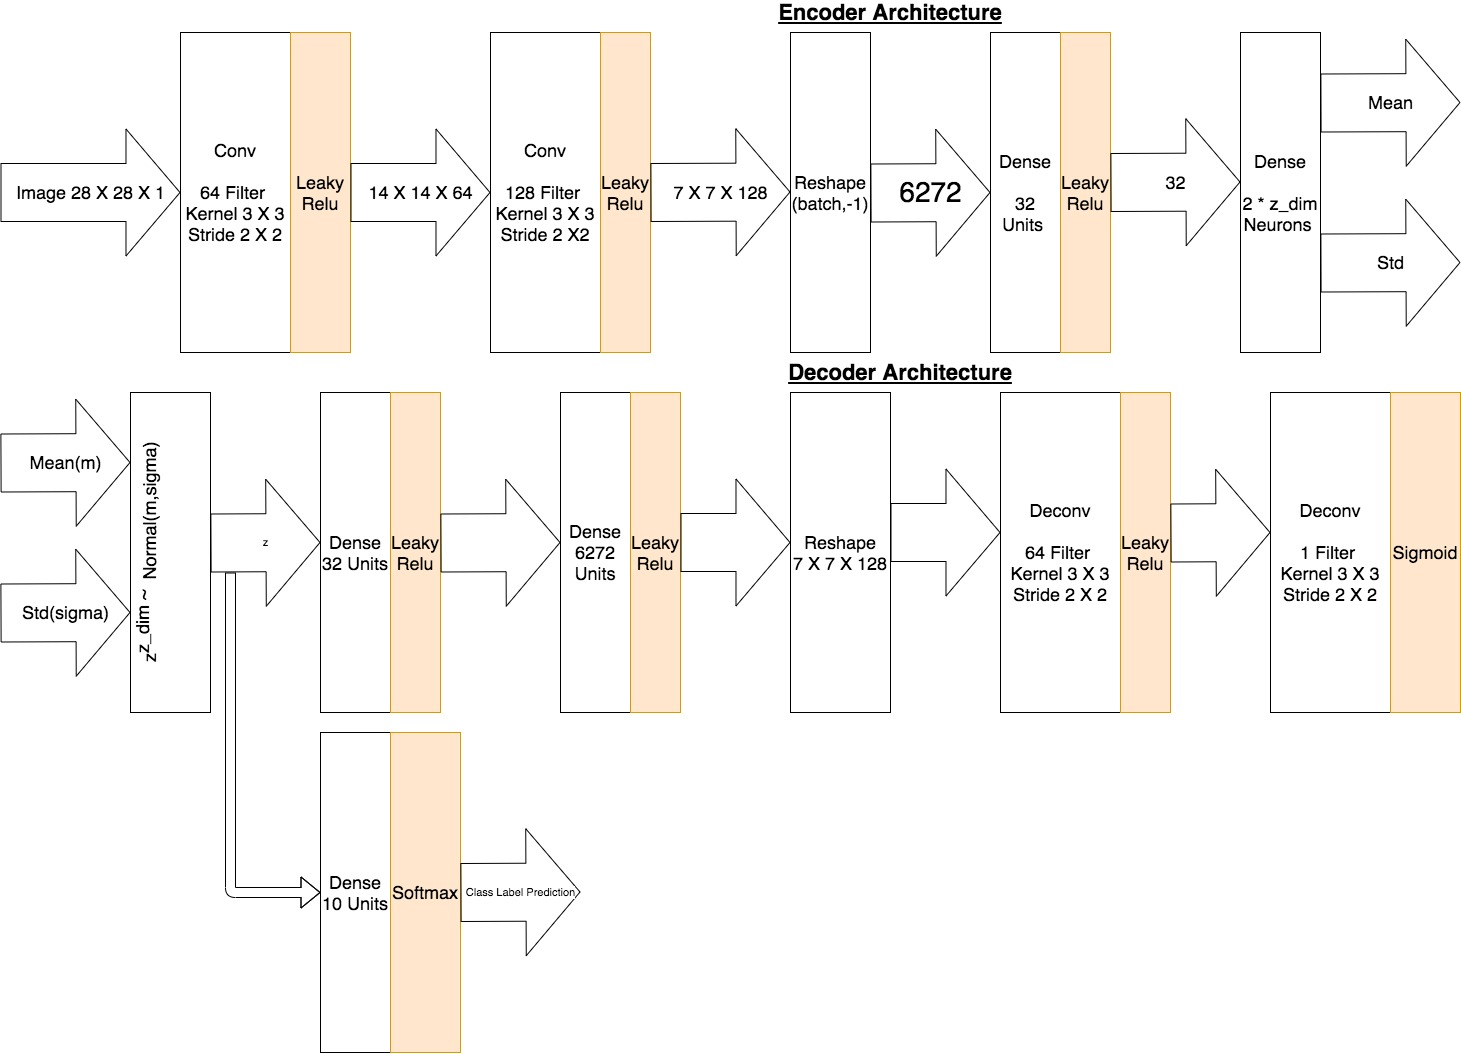
\includegraphics[width=3.5in]{vae_model_architecture_classification.jpg}
\DeclareGraphicsExtensions.
\caption{Proposed model architecture}
\label{vae_architecture}
\end{figure}

Figure \ref{vae_architecture} shows the architecture of the proposed model used with MNST dataset.
The model contains an encoder  with two down-sampling convolutional layers followed by two dense layers and decoder with two dense layers and two up-sampling de-convolution layers as in a regular VAE.
We add an additional softmax classification layer to classify the latent vectors learned by VAE into one of the 10 class labels.
We use leaky relu with a leak value of 0.2 as non-linearity for all layers. To make the network simple, there is no max-pooing layer and down-sampling is achieved by using convolution with stride of 2.
As detailed in section \ref{training} below, the network is initially trained without classification loss untill the reconstruction loss converges.
Classification loss is then added

\subsection{Loss function and training}
The variational autoencoder is initially trained until the reconstruction loss converges using the beta-VAE loss function\cite{beta_vae} given below.

\begin{equation} \label{vae_loss_eqn}
%\begin{split}
L_{VAE} = -\sum_{i, j}(x_{ij}^n \ln \hat{x}_{ij}^n
+ (1 - x_{ij}^n) \ln(1 -  \hat{x}_{ij}^n ) )\\
%+ \beta \infdiv{p(z)}{N(0,I)}
    +\beta KLD(p(z), N(0,I))
%\end{split}
\end{equation}
where   $x_{ij}$ is the pixel value at position $(i, j)$ of the input image, $\hat{x}_{ij}$ is the pixel value of reconstructed image, $p(z)$ is the probability density function of latent vectors, $N(0,I)$ is the standard multivariate normal distribution of dimension $z_{dim}$ and KLD() deontes KL divergence.
We used $\beta = 5$ as it gave the best compromise between reconstruction quality and KL divergence.
We use binary cross entropy as reconstruction loss for MNIST image, since the output activation function is sigmoid and MNIST image is treated as a binary image in our experiments.

Once a reasonably good ( goodness is measured in terms of reconstruction loss on validation data), latent representation is learned using  unsupervised beta-VAE loss function mentioned above, the latent vectors corresponding to the training samples are clustered into $k=10$ clusters.
The cluster centers were decoded using the decoder part of VAE and the resulting images corresponding to cluster centers were manually given a label and a confidence.
Figure \ref{cluster_center_1_gmm} shows the reconstructed images of cluster centers.
if the cluster center for a cluster does not correspond to any valid digit image, all the samples in that cluster is again clustered into $k$ clusters and a further attempt is made to label the cluster centers of second level cluster.
The precess can be continued to form clusters at multiple levels based on the available manual annotation budget.
The labels assigned to the cluster center is then propaged to all other samples in the cluster using the following strategy
\begin{enumerate}
    \item Each sample in the cluster is assigned with the  same label as the cluster center.
    \item Each sample is also given a confidence based on its distance from cluster center and  a manually assigned confidence in the range of [0,1]. The overall confidence of  training sample $x^n$ is computed as
\begin{equation}
w_n = p_cf(d_n)
\end{equation}
where $d_n$ is the distance of the sample from its cluster center, $p_c$  is the confidence manually assigned to the cluster center and $f: d \mapsto [0,1]$ is a monotonically decreasing function that maps distance to a confidence value in unit interval [0,1].
\end{enumerate}

\begin{figure}[]
\centering
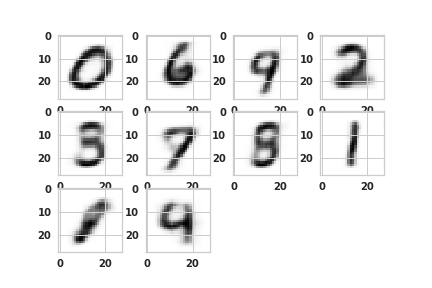
\includegraphics[width=\linewidth]{cluster_centers_epoch_1_0.png}
\caption{Images of decoded cluster center after unsupervised training using MNIST images}
\label{cluster_center_1_gmm}
\end{figure}

Experiments were performed with different choices for the distance metric(Euclidean and Mahalanobis) and confidence decay function $f$.
For the confidence decay function, we tried both the exponential decay function and gaussian function with different decay rates as given in equation \ref{exp_decay} and \ref{gaussian_decay} respectively.
We tried two different choices for distance  1) Euclidean distance and 2) Mahalanobis distance and two different choices for function $f$ 1) an exponentially decaying function and  2) a function defined by normal curve

\begin{equation}
    w_n = p_ce^{-a d_n}
    \label{exp_decay}
\end{equation}


\begin{equation}
    w_n = p_ce^{-a d_n^2}
    \label{gaussian_decay}
\end{equation}
where $a$ is a hyper parameter determining how fast the confidence decreases


Training is continued for  few more epochs using a modified loss function that incorporates the manual labels and confidence.
The modified loss function is
\begin{equation} \label{semi_supervised_loss}
L = L_{VAE}  - \gamma \sum_{k=0}^{K}w_{n}y_{n}\ln(\hat{y}_{n})
\end{equation}

where $y_n$ is the label given to the training images and $\hat{y}$ is the predicted label of the image.
The new term added to the loss is the weighted multi-class cross entropy loss for classification task.


We also performed experiments by using gmm instead of k-means for clustering.
When using gmm for clustering we directly used the product of posterior probability of the sample and cluster center confidence $p_c$ as the overall sample confidence.

As expected we obtained the best performance when using gmm.
It is also observed that when k-means is used the Mahalanobis distance along with a gaussian confidence decay function gave the best result as opposed to Euclidean distance with exponential decay of confidence


\section{Results and Discussions}
Figure \ref{classification_acc_unsupervised} shows the  classification accuracy on test dataset during the initial 10 epochs of training.
It is observed that the classification accuracy increases by about $3\%$ even without any labelled data.
From this it is evident that as the unsupervised VAE training progresses the classification accuracy also increases.
However, the increase in classification accuracy is very slow.
After epoch $10$ the semisupervised mode was started. Fig \ref{classification_acc_semi_supervised}  shows the increase in classification accuracy along with the number of samples annotated  during semisupervised training mode.

\begin{figure}[]
\centering
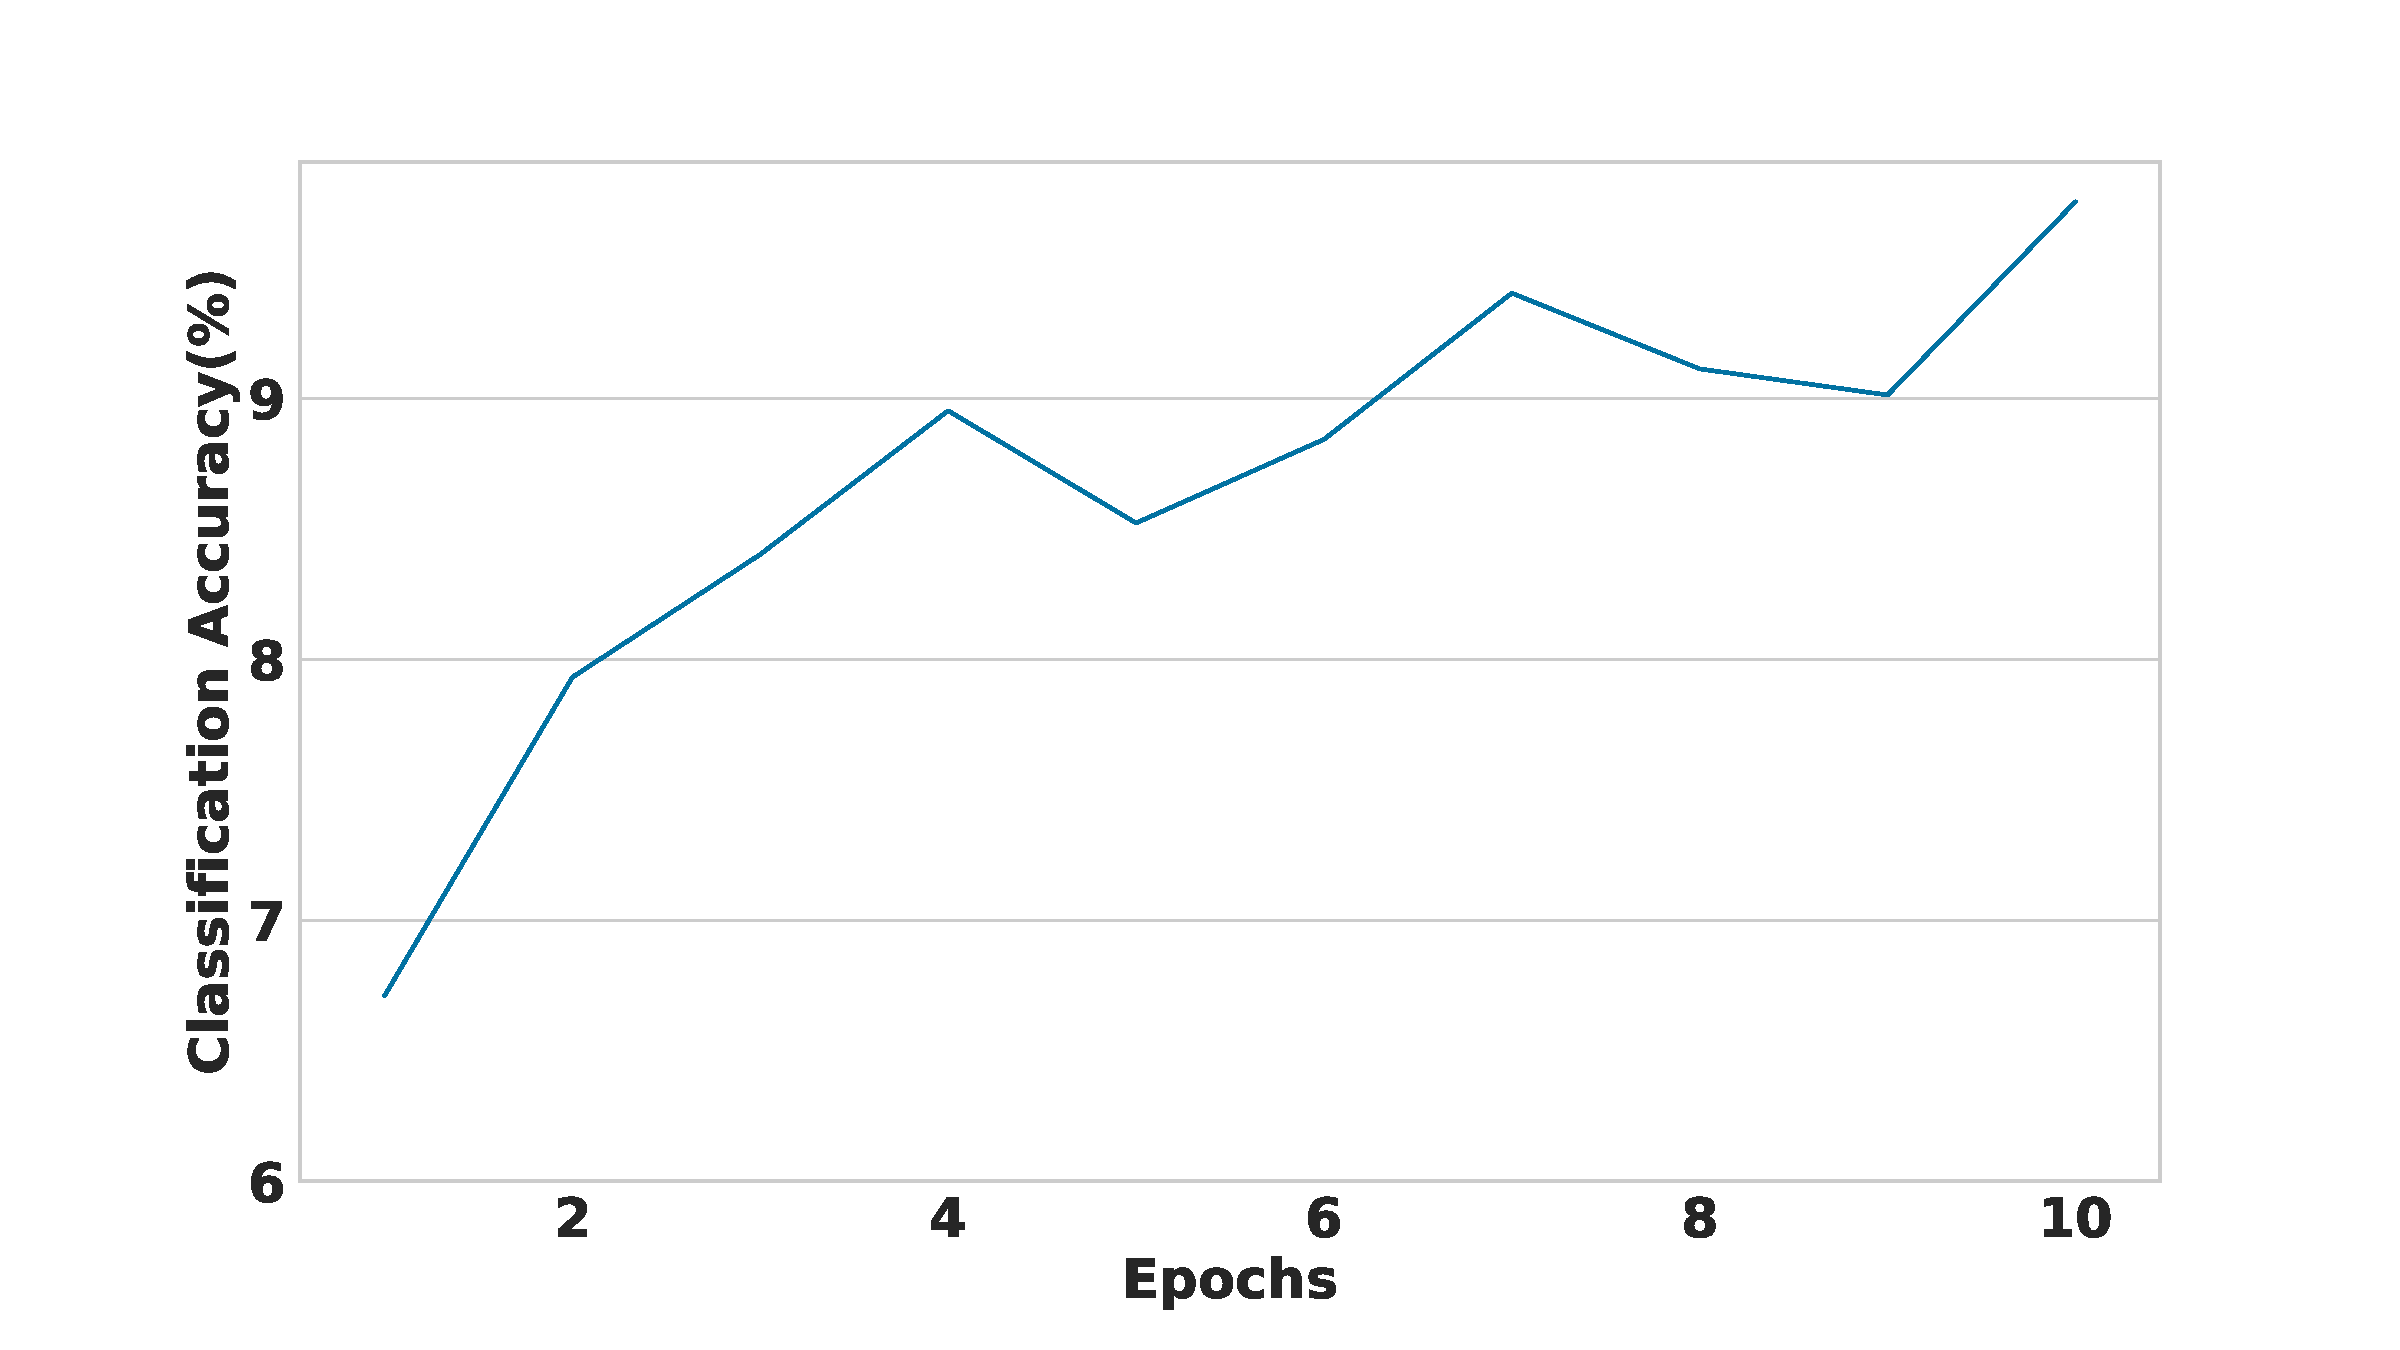
\includegraphics[width=\linewidth]{classification_acc_unsupervised}
\caption{Classification accuracy on test dataset during unsupervised training}
\label{classification_acc_unsupervised}
\end{figure}

\begin{figure}[]
\centering
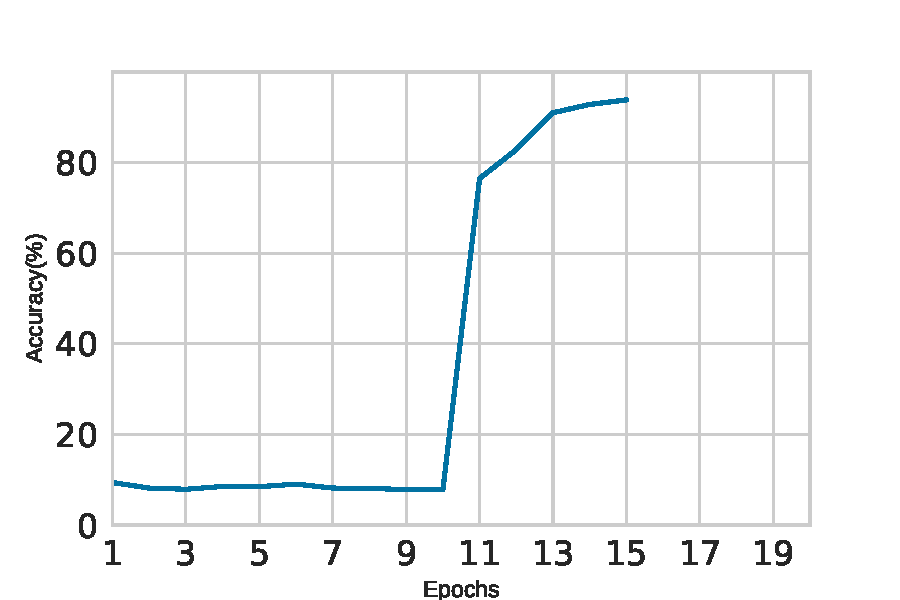
\includegraphics[width=\linewidth]{classification_acc_semi_supervised}
\caption{Classification accuracy on test dataset during semisupervised training. The semisuprevised mode starts after epoch 10}
\label{classification_acc_semi_supervised}
\end{figure}


\section{Conclusion}
%
% ---- Bibliography ----
%
% BibTeX users should specify bibliography style 'splncs04'.
% References will then be sorted and formatted in the correct style.
%
% \bibliographystyle{splncs04}
% \bibliography{mybibliography}
%
\begin{thebibliography}{8}
    \bibitem{beta_vae}
    Higgins, Irina, et al. "beta-vae: Learning basic visual concepts with a constrained variational framework." (2016)
\end{thebibliography}
\end{document}
